\documentclass[dvipdfmx]{beamer}
\usepackage{bxdpx-beamer}% dvipdfmxなので必要
\usepackage{pxjahyper}% 日本語で'しおり'したい
%\usepackage{etex}
%\usetheme{Warsaw}
\usetheme{Malmoe}
%\usetheme{AnnArbor}
%\usetheme{Hannover}
%\usetheme{Bergen}
%\usetheme{Berlin}
%\usetheme{Singapore}
%\usetheme{Montpellier}
%\usetheme{Pittsburgh}
\usepackage{graphicx}
\usepackage{latexsym,amssymb}
%\usepackage{epsbox}
%\usepackage{multirow}
\usepackage{fancybox}
\usepackage{fancyvrb}
%\usepackage{listings}
\usepackage{tabularx}
\usepackage{tikz}
\usetikzlibrary{calc,shapes}
%\usepackage{pstricks,pst-node,pst-tree}
%\usepackage{multimedia}
%\usepackage{pstricks,pst-node,pst-tree}
%\usepackage{pst-all}
%\include{prooftree}
%\lstloadlanguages{pascal}
\renewcommand{\kanjifamilydefault}{\gtdefault}
\renewcommand{\familydefault}{\sfdefault}

\graphicspath{{fig251111/}}

%\include{cmacros}

\newcommand{\greentext}[1]{{\color[rgb]{0,0.5,0}{#1}}}
\newcommand{\redtext}[1]{{\color[rgb]{0.8,0,0}{#1}}}
\newcommand{\bluetext}[1]{{\color[rgb]{0,0,0.8}{#1}}}

\newcommand{\tuple}[1]{\langle{#1}\rangle}

\newcommand{\First}{\mathsf{First}_1}
\newcommand{\Follow}{\mathsf{Follow}_1}

%%pdt simulation

\newcommand{\pdtline}[6]{%
    \uncover<#6->{
    \node at (${#5}*(0,-.3)+(0,.3)$) {$\vdash$};%
    \node at (${#5}*(0,-.3)+(1.5,.3)$) {\parbox{12em}{(#1,}};%
    \node at (${#5}*(0,-.3)+(4.5,.3)$) {\parbox{10em}{#2,}};%
    \node at (${#5}*(0,-.3)+(5.7,.3)$) {\parbox{10em}{#3)}};%
    \node at (${#5}*(0,-.3)+(8,.3)$) {\parbox{20em}{#4}};%
    }
}

\newcommand{\initpdtline}[6]{%
    \uncover<#6->{
    \node at (${#5}*(0,-.3)+(1.5,.3)$) {\parbox{12em}{(#1,}};%
    \node at (${#5}*(0,-.3)+(4.5,.3)$) {\parbox{10em}{#2,}};%
    \node at (${#5}*(0,-.3)+(5.7,.3)$) {\parbox{10em}{#3)}};%
    \node at (${#5}*(0,-.3)+(8,.3)$) {\parbox{20em}{#4}};%
    }
}

\newtheorem{Def}{定義}
\newtheorem{Lem}{補題}
\newtheorem{Thm}{定理}
\newtheorem{Prop}{命題}

\definecolor{lightlightgrey}{rgb}{0.95,0.95,0.95}



%\newcommand{\greentext}[1]{{\color[rgb]{0,0.5,0}{#1}}}
%\newcommand{\redtext}[1]{{\color[rgb]{0.8,0,0}{#1}}}

\newcommand{\lecturedate}{2025/11/11}

\cornersize{0.25}

\setbeamertemplate{frametitle}[default][center]
\setbeamertemplate{footline}{\hfill
コンパイラ\quad\lecturedate
\hfill\insertframenumber/\inserttotalframenumber\hspace*{1zw}}
\newcounter{coffee}
\setbeamercovered{transparent=10}
\title{コンパイラ(12)}
\date{\lecturedate}
\begin{document}

\frame{\titlepage}



\subsection{大域的最適化}
 
 \begin{frame}
 \frametitle{大域的コード最適化}
 基本ブロックを越える最適化

 \begin{list}{}{}
  \item ループ最適化
  \item 手続き呼び出し最適化
  \item データフロー解析
  \item 静的単一代入(SSA)解析
 \end{list}
\end{frame}

\begin{frame}
 \frametitle{ループ最適化(1/3)}
 ループ内のコード実行回数:ループ外のコードよりも一般に多い\\
 ループ内のコードは慎重に最適化\\
 本当に毎回実行しなければならないか？できるだけ効率よく実行
 \begin{list}{}{}
  \item ループ不変式の移動\\
	\greentext{ループから影響をうけない式を外に出す}l\\
	例6.8
  \item ループ内の演算の強さの軽減\\
	強い演算：時間のコストが大きい演算\\
	足し算$<$掛け算 (加算器$<$乗算器)\\
	例6.9
 \end{list}
\end{frame}

\begin{frame}
 \frametitle{例}
 \begin{center}
 \begin{tabular}{ccc}
  \multicolumn{3}{l}{例6.8}\\
  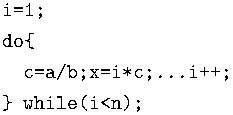
\includegraphics[scale=.7]{ex6_8_1.pdf}
  & $\Rightarrow$ & 
  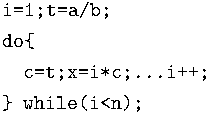
\includegraphics[scale=.7]{ex6_8_2.pdf} \\[1zw]
  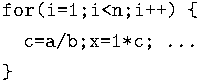
\includegraphics[scale=.7]{ex6_8_3.pdf}
  & $\Rightarrow$ & 
  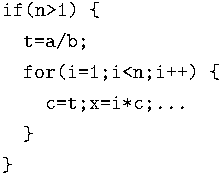
\includegraphics[scale=.7]{ex6_8_4.pdf} \\[1zw]
  \multicolumn{3}{l}{例6.9}\\
  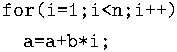
\includegraphics[scale=.7]{ex6_9_1.pdf}
  & $\Rightarrow$ & 
  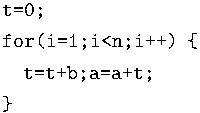
\includegraphics[scale=.7]{ex6_9_2.pdf}
 \end{tabular}
 \end{center}
\end{frame}

\begin{frame}
 \frametitle{ループ最適化(2/3)}
 \begin{list}{}{}
  \item 帰納変数消去\\
	\greentext{帰納変数(ループを制御する変数)は減らす。}\\
	\greentext{参照数の減少}
	\begin{center}
	 \begin{tabular}{ccc}
	  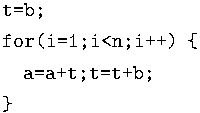
\includegraphics[scale=.75]{ex6_10_1.pdf}
	  & $\Rightarrow$ &
	  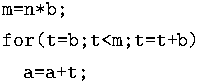
\includegraphics[scale=.75]{ex6_10_2.pdf}
	 \end{tabular}
	\end{center}
	
  \item ループ融合とループ分離\\
  \item ループ展開とソフトウェアパイプライン
 \end{list}
\end{frame}

\begin{frame}
 \frametitle{ループ展開とソフトウェアパイプライン}
 \begin{center}
 \begin{tabular}{ccc}
  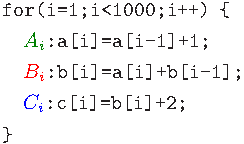
\includegraphics[scale=.75]{ex6_14_1.pdf}
  & $\Rightarrow$ &
  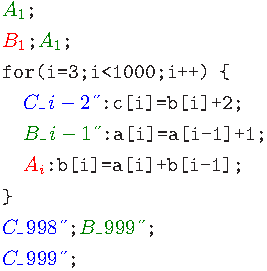
\includegraphics[scale=.75]{ex6_14_2.pdf}
 \\
 \end{tabular}

  \[
   \begin{array}{c|ccc}
    &P_1 &P_2 &P_3 \\\hline
   1 & A_1 & & \\
   2 & B_1 & A_2 & \\
   3 & C_1 & B_2 & A_3 \\
   4 & A_4 & C_2 & B_3 \\
   5 & B_4 & A_5 & C_3 \\
   \vdots & \multicolumn{3}{c}{\vdots}\\
   \end{array}
  \]
 並列に実行可能
 \end{center}
\end{frame}

\begin{frame}
 \frametitle{手続き呼出し最適化}

 \begin{list}{}{}
  \item {\bf インライン展開}:\ \\
 手続き呼出し=駆動レコードを用いてスタック上に情報を保存

 \greentext{操作としてはコストが大きい}

 スタック操作：実メモリへの正確な順序での書き込みを要求

 短い手続きや関数であればそのまま置き換えてしまった方が
 効率がよい。

  \item {\bf 末尾再帰}:\\

	手続の最後の再帰よびだしは、gotoに置き換え可能。
	
	\greentext{呼出しから復帰しても駆動レコード上の局所環境を使って
	実行する命令が存在しない。局所領域も再利用可能}
 \end{list}

\end{frame}

\begin{frame}
 \frametitle{末尾再帰の例}
 \begin{tabular}{ccc}
  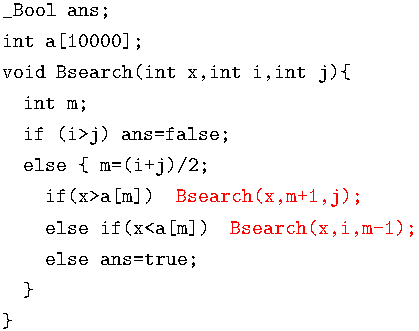
\includegraphics[scale=.6]{ex6_16_1.pdf}
  & $\Rightarrow$ &
  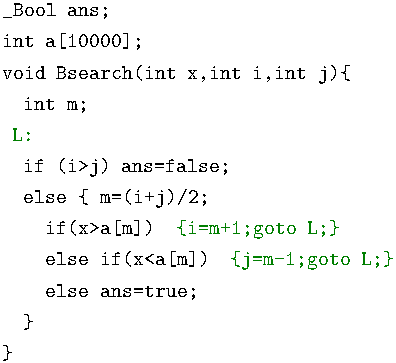
\includegraphics[scale=.6]{ex6_16_2.pdf}\\
  & & $\Downarrow$\\
  & &
  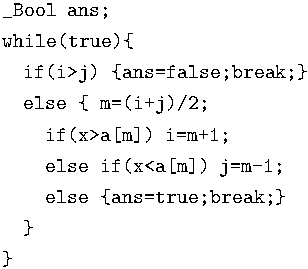
\includegraphics[scale=.6]{ex6_16_3.pdf}
 \end{tabular}
\end{frame}

\subsection{データフロー解析}

\begin{frame}
 \frametitle{データフロー解析}

 \vspace*{10pt}

 \greentext{(講義資料6.4:詳細については省略)}

 \vspace*{10pt}

 基本ブロック$B$に対するデータフロー

 \[
  out[B]=gen[B]\cup(in[B]-kill[B])
 \]

 プログラム上での位置(行番号)：
 \begin{tabular}{ll}
  $in[B]$ & $B$に入力されるデータ\\
  $out[B]$ & $B$から出力されるデータ\\
  $gen[B]$ & $B$で定義されるデータ\\
  $kill[B]$ & $B$で上書きされるデータ\\
 \end{tabular}

 入力から出力への制御がきまっていればよいので、基本ブロック単位で考えれ
 ばよい。

 ループ：データフロー方程式を解いて全体的に必要なデータを計算する。
\end{frame}

\begin{frame}{データフロー方程式}
% \begin{tabular}{ccc}
%  \begin{minipage}{.2\textwidth}
% \begin{tikzpicture}
%  \node[draw] (S1) at (0,1.5) {$S_1$};
%  \node[draw] (S2) at (0,0) {$S_2$};
%  \path[->] (S1) edge (S2);
% \end{tikzpicture}
%  \end{minipage}
%  &
%  \begin{minipage}{.25\textwidth}
%   \begin{tikzpicture}
%    
%   \end{tikzpicture}
%  \end{minipage}
% \end{tabular}

\greentext{定義到達可能性解析：}

\scalebox{0.7}{
\begin{tikzpicture}
 \node[draw] (B5) at (2,0) {EXIT};
 \node[draw] (B4) at (2,1.25) {$\begin{array}{ll}d_7: &
  \texttt{i=u3}\\ & \texttt{if...}\end{array}$};
 \node[draw] (B3) at (0,2.25) {$d_6$:\texttt{a=u2}};
 \node[draw] (B2) at (2,3.5) {$\begin{array}{ll}
  d_4: & \texttt{i=i+1}\\[-3pt]
  d_5: & \texttt{j=j-1}\\[-3pt]
  & \texttt{if ...}
		       \end{array}$};
 \node[draw] (B1) at (2,5.25) {$\begin{array}{ll}
  d_1: & \texttt{i=m-1}\\[-3pt]
  d_2: & \texttt{j=n}\\[-3pt]
  d_3: & \texttt{a=u1}
			\end{array}$};
 \node[draw] (B0) at (2,6.75) {ENTRY};

 \node at ($(B1)+(1.75,0)$) {$B_1$};
 \node at ($(B2)+(1.75,0)$) {$B_2$};
 \node at ($(B3)+(1.2,0)$) {$B_3$};
 \node at ($(B4)+(1.75,0)$) {$B_4$};

 \path[->] (B0) edge (B1) (B1) edge (B2) (B2) edge (B4)
           (B2) edge (B3) (B3) edge (B4) (B4) edge (B5);
 \path[->] (B4) [out=210,in=150,looseness=3] edge (B2);

 \node[anchor=west] at ($(B1)+(2.5,0)$) {$\begin{array}{ll}
  gen_{B_1} & = \{d_1,d_2,d_3\}\\[-3pt]
  kill_{B_1} & = \{d_4,d_5,d_6,d_7\}
			   \end{array}$};
 \node[anchor=west] at ($(B2)+(2.5,0)$) {$\begin{array}{ll}
  gen_{B_2} & = \{d_4,d_5\} \\[-3pt]
  kill_{B_2} & = \{d_1,d_2,d_7\}
			   \end{array}$};
 \node[anchor=west] at ($(B3)+(4.5,0)$) {$\begin{array}{ll}
  gen_{B_3} & = \{d_6\}\\[-3pt]
  kill_{B_3} & = \{d_3\}
			   \end{array}$};
 \node[anchor=west] at ($(B4)+(2.5,0)$) {$\begin{array}{ll}
  gen_{B_4} & = \{d_7\} \\[-3pt]
  kill_{B_4} & = \{d_1,d_4\}
			   \end{array}$};
\end{tikzpicture}
}

\vspace*{-30pt}

{\footnotesize
\begin{eqnarray*}
 IN[B_2] & = & OUT[B_1]\cup OUT[B_4]\\
 OUT[B_2] & = & gen_{B_2}\cup(IN[B_2]-kill_{B_2})
\end{eqnarray*}
}

(Ahoら：Compilers より引用)
\end{frame}

\begin{frame}
  \frametitle{データフロー方程式}
  \[
    \begin{array}{rcl}
      OUT[B_1]& = & gen_{B_1}\\
      IN[B_2] & = & OUT[B_1]\cup OUT[B_4]\\
      OUT[B_2] & = & gen_{B_2}\cup(IN[B_2]-kill_{B_2})\\
      IN[B_3] & = & OUT[B_2]\\
      OUT[B_3] & = & gen_{B_3}\cup(IN[B_3]-kill_{B_3})\\
      IN[B_4] & = & OUT[B_3]\cup OUT[B_2]\\
      OUT[B_4] & = & gen_{B_4}\cup(IN[B_4]-kill_{B_4})
    \end{array}
    \]
\end{frame}

\begin{frame}{データフロー方程式の計算}

到達可能性解析：

{\small
{XXXX XXX}:$d_1,d_2,\cdots,d_7$が集合に入っているとき$1$、入ってないとき$0$
}

\vspace*{10pt}

{\footnotesize
\begin{tabular}{c|c|c|c|c|c}\hline
Block $B$ & OUT[$B$]$^0$ & IN[$B$]$^1$ & OUT[$B$]$^1$ & IN[$B$]$^2$ & OUT[$B$]$^2$\\\hline
$B_1$ & 111 0000 & 000 0000 & 111 0000 & 000 0000 & 111 0000\\
$B_2$ & 000 1100 & 111 0001 & 001 1100 & 111 0111 & 001 1110\\
$B_3$ & 000 0010 & 000 1100 & 000 1110 & 001 1100 & 000 1110\\
$B_4$ & 000 0001 & 000 1110 & 000 0111 & 001 1110 & 001 0111\\\hline
\end{tabular}
}

\vspace*{10pt}

\greentext{変化しなくなるまでくりかえす。}


$OUT[B_4]$=001 0111:\\
\greentext{本ブロックでは$d_3$,$d_5$,$d_6$,$d_7$がEXITが到達する可能性がある．}

\end{frame}

\begin{frame}
  \frametitle{データフロー}
  \greentext{生存解析}
  \begin{tabular}{ll}
  $Use[B]$: & $B$で再定義される前に資料される変数の集合\\
  $Def[B]$: & $B$で定義される変数の集合
  \end{tabular}

  \begin{eqnarray*}
    In[B] & = & Use[B]\cup(Out[B]-Def[B])\\
    Out[B] & = & \cup_{S\in Succ[B]}In[S]
  \end{eqnarray*}
  $Succ[B]$: フローグラフにおいて$B$から直接フローがあるブロック
\end{frame}

\begin{frame}
  \frametitle{データフロー解析}
  \scalebox{0.7}{
\begin{tikzpicture}
 \node[draw] (B5) at (2,0) {EXIT};
 \node[draw] (B4) at (2,1.25) {$\begin{array}{ll}d_7: &
  \texttt{i=u3}\\ & \texttt{if...}\end{array}$};
 \node[draw] (B3) at (0,2.25) {$d_6$:\texttt{a=u2}};
 \node[draw] (B2) at (2,3.5) {$\begin{array}{ll}
  d_4: & \texttt{i=i+1}\\[-3pt]
  d_5: & \texttt{j=j-1}\\[-3pt]
  & \texttt{if ...}
		       \end{array}$};
 \node[draw] (B1) at (2,5.25) {$\begin{array}{ll}
  d_1: & \texttt{i=m-1}\\[-3pt]
  d_2: & \texttt{j=n}\\[-3pt]
  d_3: & \texttt{a=u1}
			\end{array}$};
 \node[draw] (B0) at (2,6.75) {ENTRY};

 \node at ($(B1)+(1.75,0)$) {$B_1$};
 \node at ($(B2)+(1.75,0)$) {$B_2$};
 \node at ($(B3)+(1.2,0)$) {$B_3$};
 \node at ($(B4)+(1.75,0)$) {$B_4$};

 \path[->] (B0) edge (B1) (B1) edge (B2) (B2) edge (B4)
           (B2) edge (B3) (B3) edge (B4) (B4) edge (B5);
 \path[->] (B4) [out=210,in=150,looseness=3] edge (B2);

 \node[anchor=west] at ($(B1)+(2.5,0)$) {$\begin{array}{ll}
  Def_{B_1} & = \{i,j,a\}\\[-3pt]
  Use_{B_1} & = \{m,n,u_1\}
			   \end{array}$};
 \node[anchor=west] at ($(B2)+(2.5,0)$) {$\begin{array}{ll}
  Def_{B_2} & = \{i,j\} \\[-3pt]
  Use_{B_2} & = \{i,j\}
			   \end{array}$};
 \node[anchor=west] at ($(B3)+(4.5,0)$) {$\begin{array}{ll}
  Def_{B_3} & = \{a\}\\[-3pt]
  Use_{B_3} & = \{u2\}
			   \end{array}$};
 \node[anchor=west] at ($(B4)+(2.5,0)$) {$\begin{array}{ll}
  Def_{B_4} & = \{i\} \\[-3pt]
  Use_{B_4} & = \{u3\}
			   \end{array}$};
\end{tikzpicture}
}
\end{frame}

\begin{frame}
  \frametitle{データフロー解析（生存解析）}
  $(a,i,j,m,n,u1,u2,u3)$とすると

  {\scriptsize
  $\begin{array}{l|llllll}
     & OUT & IN & OUT & IN & OUT & IN\\\hline
  B_1 & (00000000) & (00011100) & (01100000) & (00011100) & (01100010) & (00011100)\\
  B_2 & (00000000) & (01100000) & (01100010) & (01100010) & (01100001) & (01100010)\\
  B_3 & (00000000) & (00000010) & (00000001) & (00000010) & (00100001) & (10100001)\\
  B_4 & (00000000) & (00000001) & (01100000) & (00100001) & (01100010) & (00100001)
  \end{array}$}

  \vspace*{10pt}

  \greentext{\small フローグラフの基本ブロックにおいてどの変数が影響をうけるかを解析}

  \vspace*{10pt}

  $\begin{array}{l|ll}
    & IN & OUT\\\hline
    B_1 & \{m,n,u1\} & \{i,j,u2\}\\
    B_2 & \{i,j,u2\} & \{i,j,u3\}\\
    B_3 & \{a,j,u3\} & \{j,u3\}\\
    B_4 & \{j,u3\} & \{i,j,u2\}
  \end{array}$
\end{frame}

\subsection{静的単一代入}

\begin{frame}
  \frametitle{静的単一代入を用いた最適化}
 
  データフロー解析のもうひとつの手法:
  静的単一代入(Static Single Assignment:SSA)\\
  \redtext{各変数の定義がプログラム中で唯一}
  
  変数の値は変わらないとする。二度目の代入が発生すると変数名を変更\\
 % \quad\greentext{変数を見ればUdチェーンがすぐに判明する。}\\
  \quad\greentext{値が同じの共通部分式が判別できる=式として一致}
 
  変換例：例6.20、6.21\\
  定義ごとに変数に添字をつける。合流する場合は、$\phi$関数で表現
 
  いかにして、SSA形式を得るか？
  \begin{list}{}{}
   \item [(1)] $\phi$関数の挿入
   \item [(2)] 変数の添字の決定
  \end{list}
  SSA形式において最適化
  \begin{list}{}{}
   \item [(3)] SSAから逆変換する。($\phi$関数の消去)
  \end{list}
 
  近年のコンパイラでよく用いられる手法
  
 \end{frame}
 
 \begin{frame}
  \frametitle{例}
 
  \begin{center}
  \begin{tabular}{c}
  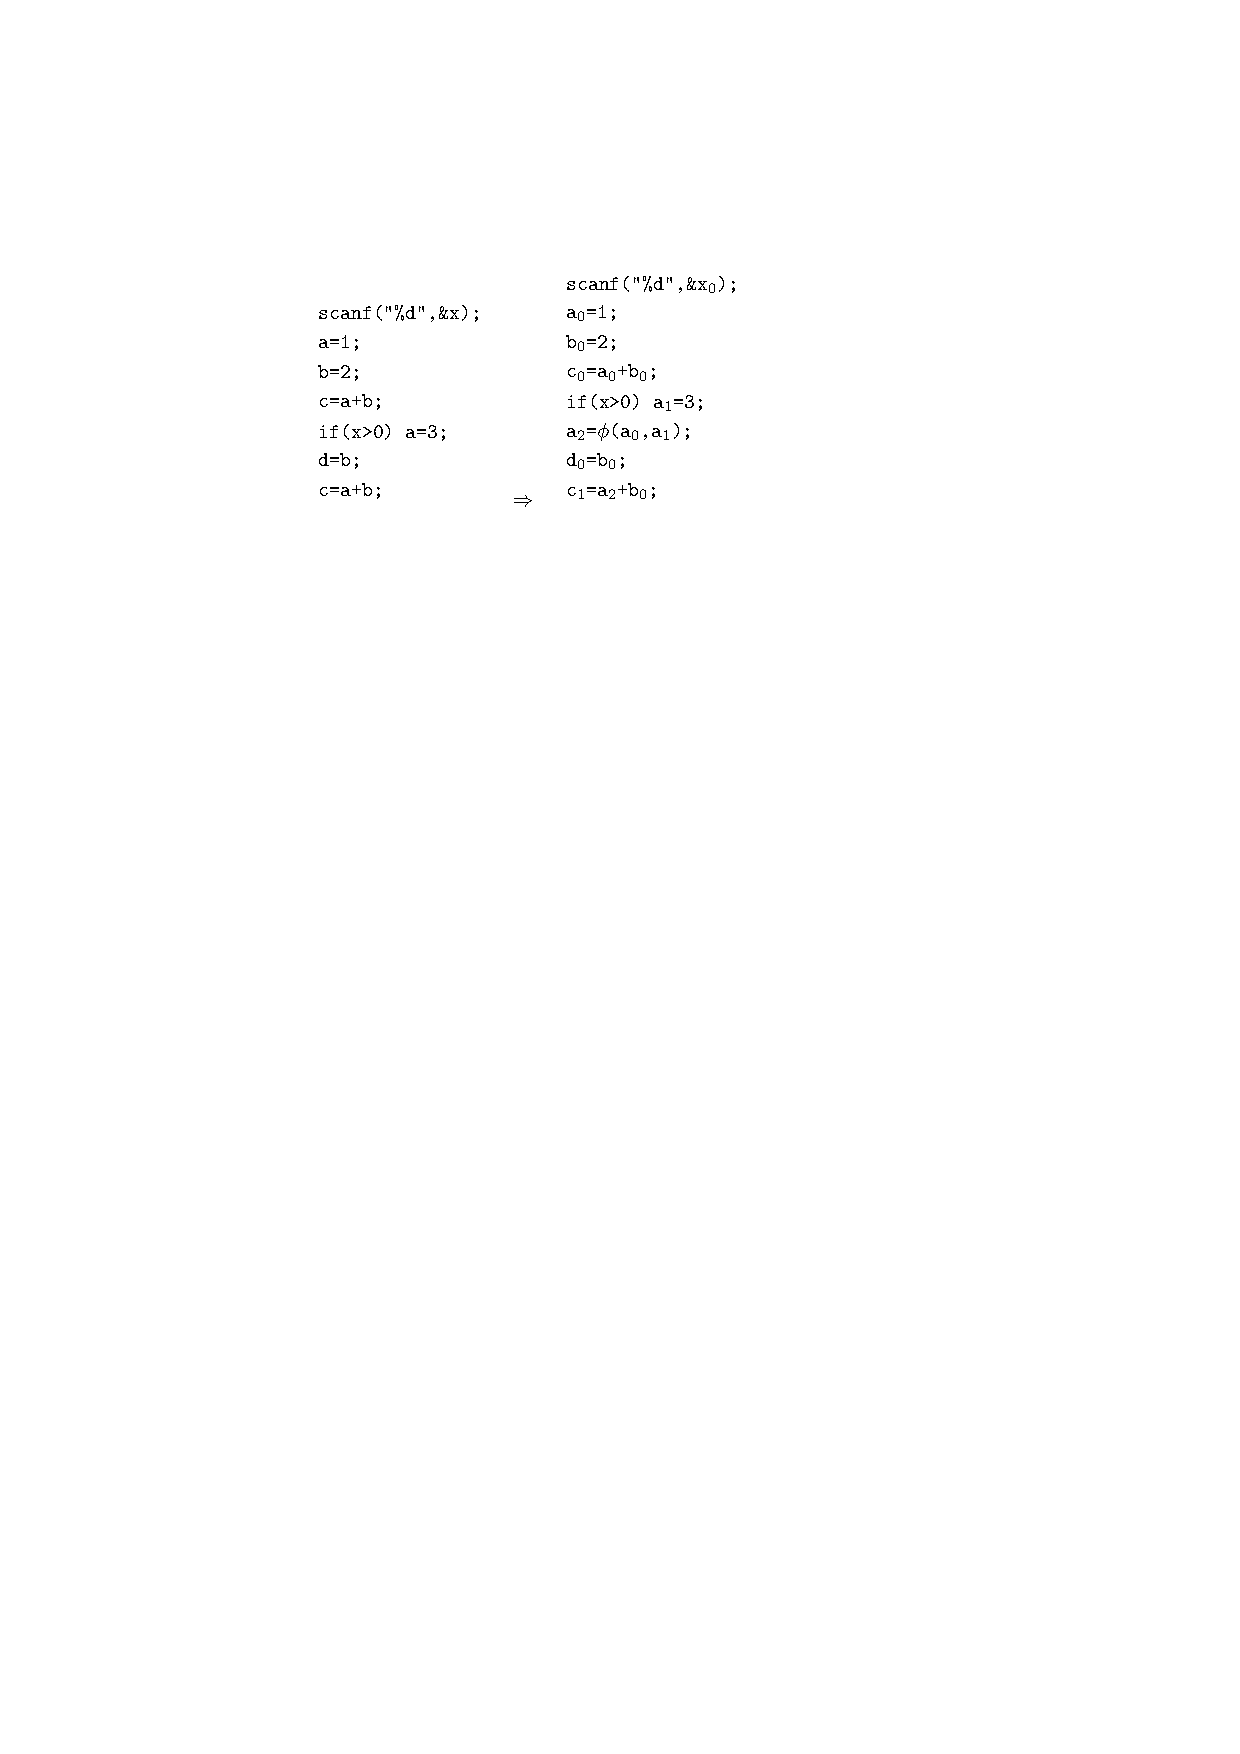
\includegraphics[height=.4\textheight]{ex6_20r1.pdf}
   \\
  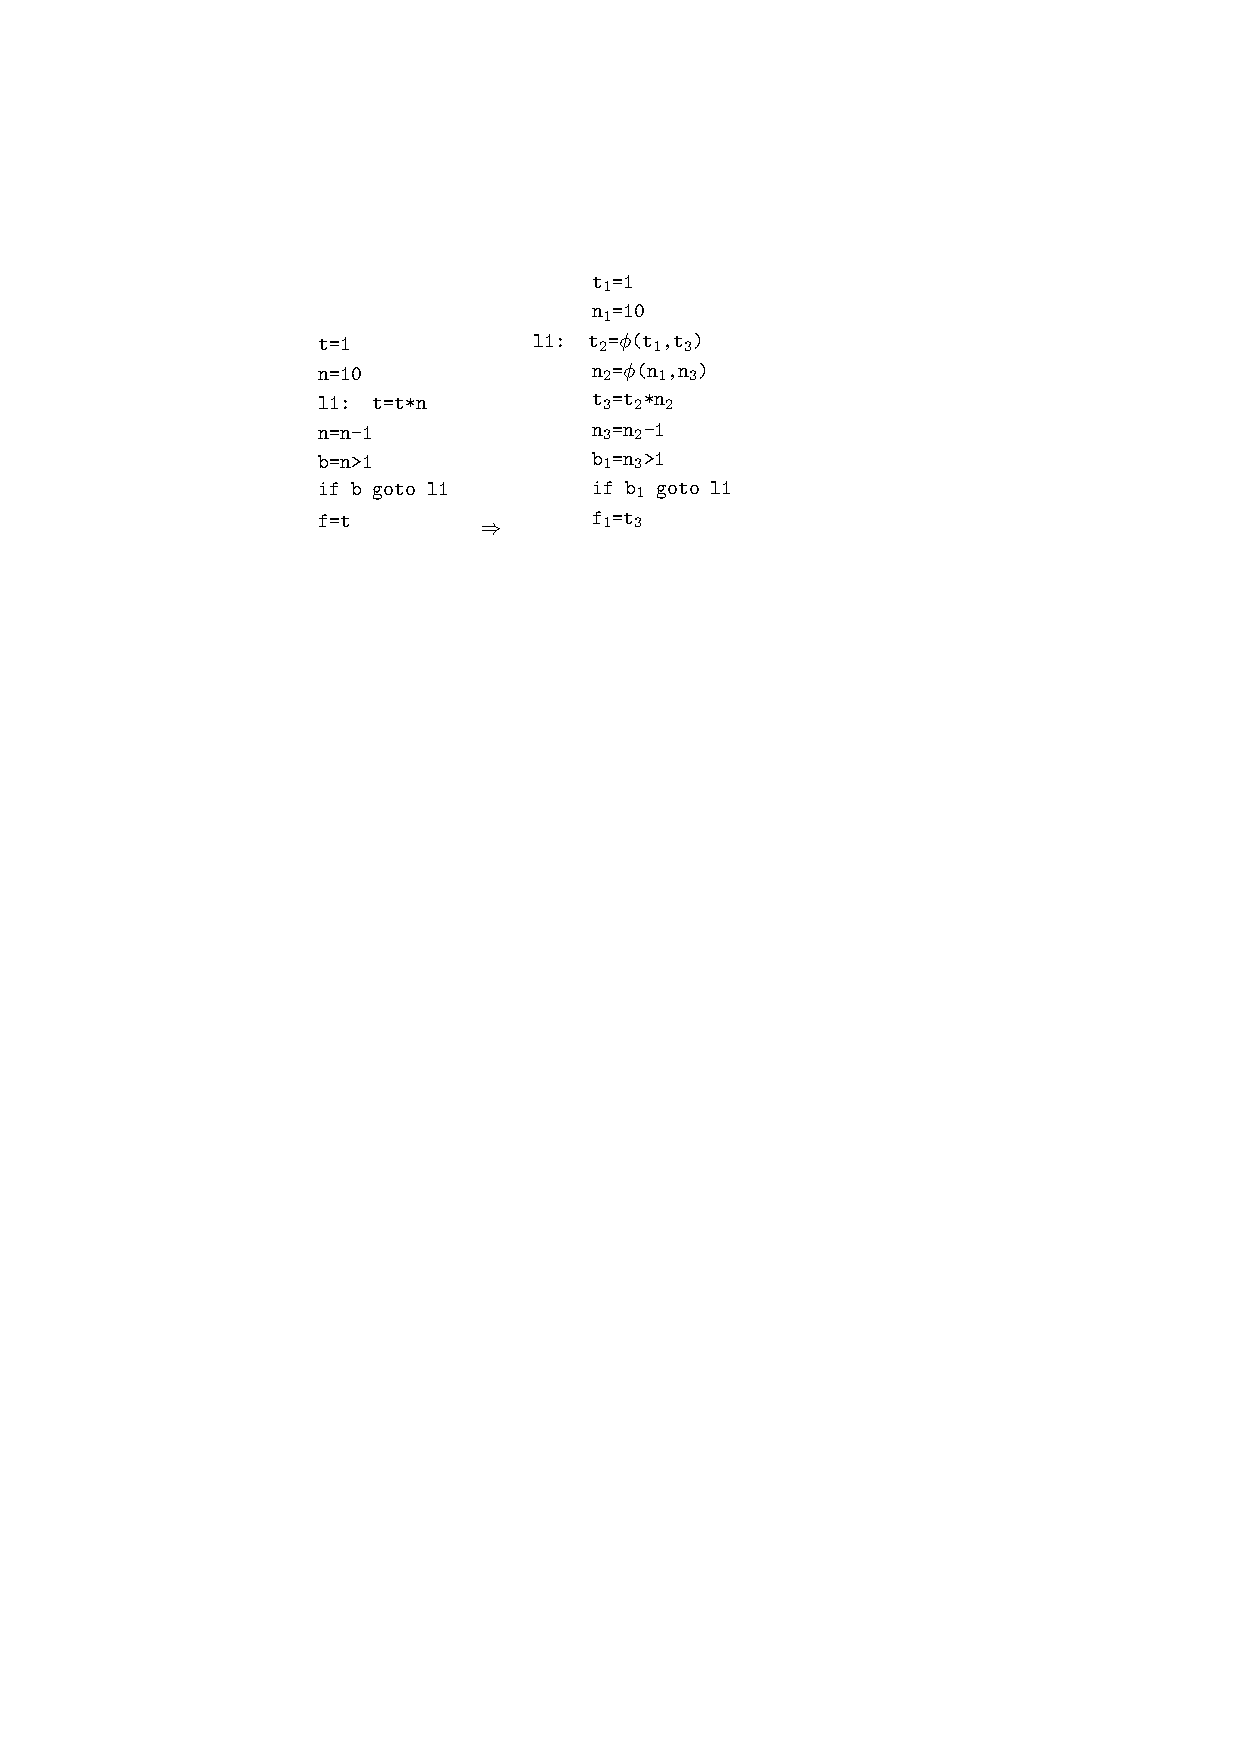
\includegraphics[height=.4\textheight]{ex6_21r1.pdf}
  \end{tabular}
  \end{center}
 \end{frame}
 
 \begin{frame}
  \frametitle{$\phi$関数の挿入}
 
  根つきグラフ：$(V,E)$ 先行頂点を持たない唯一の接点$v_o$(根)が存在
  
  \begin{center}
   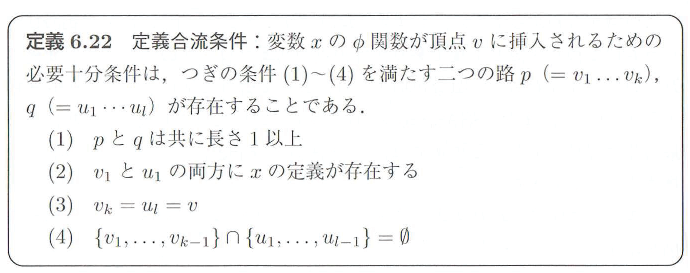
\includegraphics[width=\textwidth]{def6_22.pdf}
  \end{center}
 
  パス$p$上の$x$の定義=$x_1$,$q$上の$x$の定義=$x_2$
 定義合流条件の$v$に、$x_3=\phi(x_1,x_2)$
 \end{frame}
 
 \begin{frame}
  \frametitle{定義合流条件}
  \begin{center}
   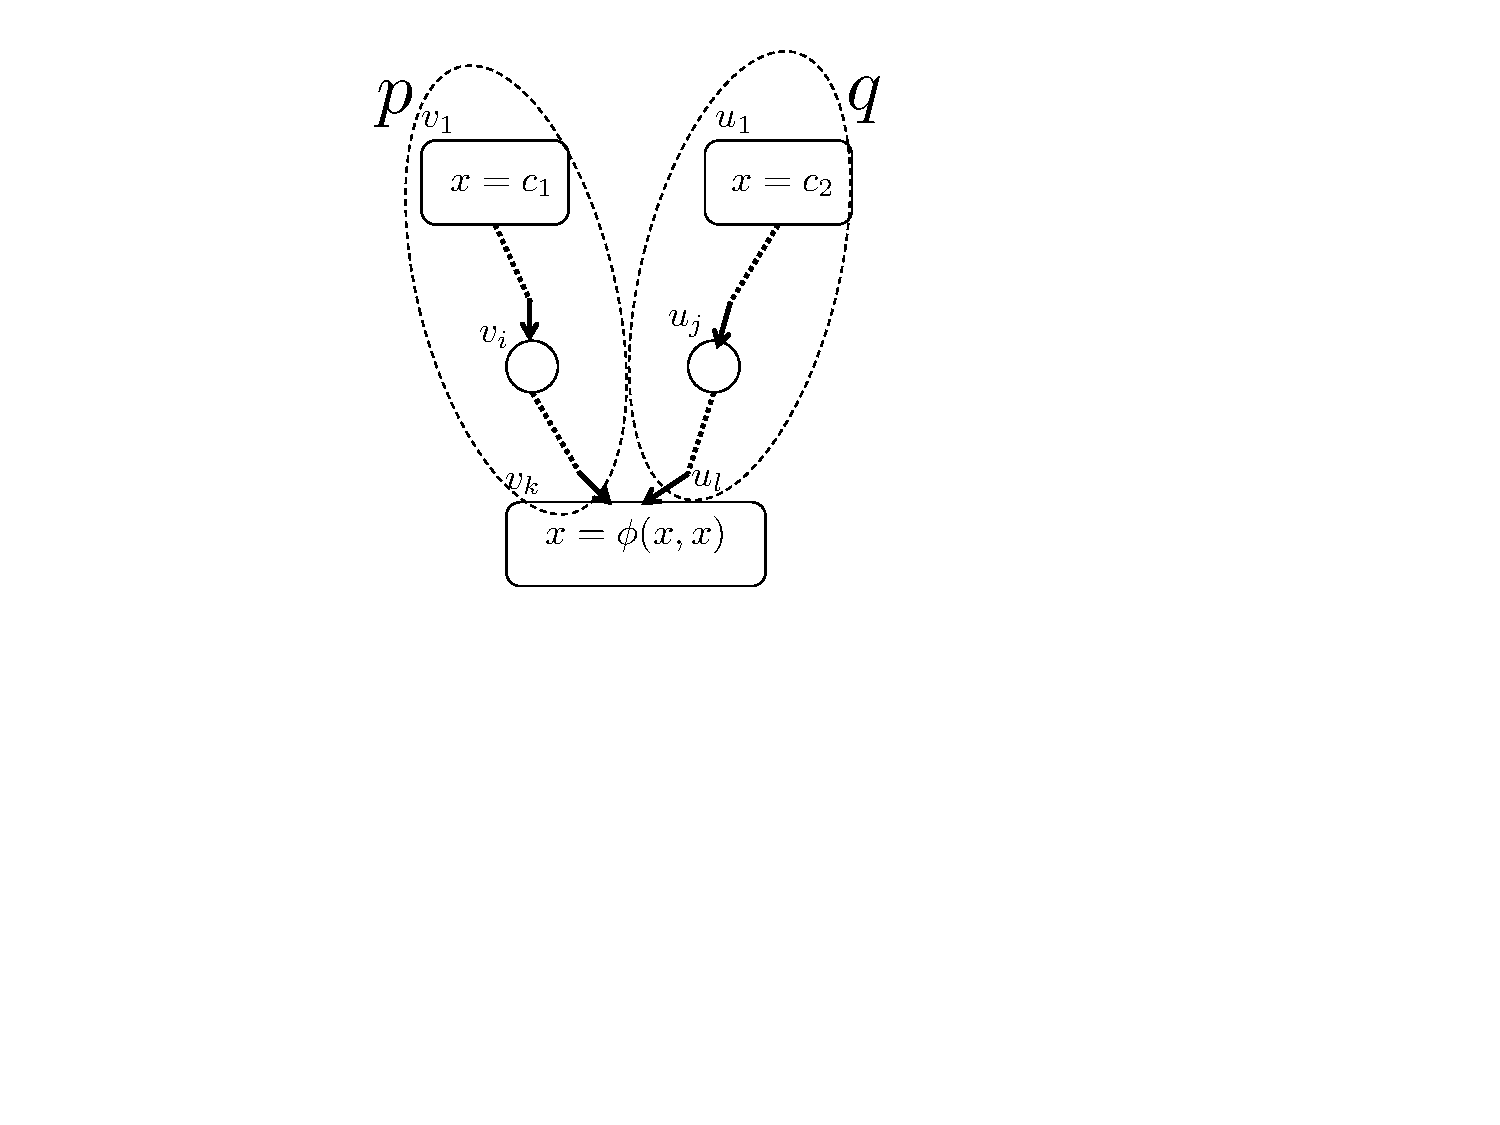
\includegraphics[width=.5\textwidth]{confluenceCondition.pdf}
  \end{center}
 \end{frame}
 
 \begin{frame}
  \frametitle{支配関係}
 
  支配関係：開始頂点からのパスに必ず含まれるとき、「支配」される。
 
  \only<1>{
  \begin{center}
   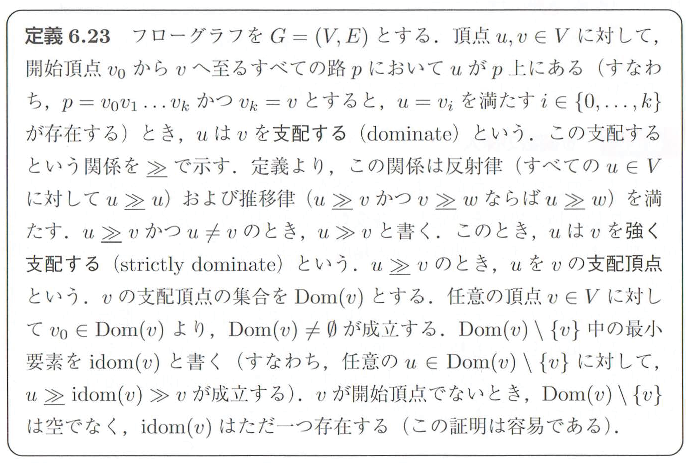
\includegraphics[width=.7\textwidth]{def6_23.pdf}
  \end{center}
 
  $u\underline{\gg}v$:$u$が$v$を支配:支配関係の表現=支配木 (図6.7)
 }
  \only<2>{
  \begin{center}
  \begin{tabular}{cc}
 
   \begin{tikzpicture}
    \node[draw,circle] (v0) at (0,3) {$v_0$};
    \node[draw,circle] (u) at (0,1.5) {$u$};
    \node[draw,circle] (v) at (0,0) {$v$};
    \node at (0,2.25) {$\cdots$};
    \node at (0,0.75) {$\cdots$};
    \path[->] (v0) [out=-30,in=30] edge (u);
    \path[->] (v0) [out=-60, in=60] edge (u);
    \path[->] (v0) [out=240,in=120] edge (u);
    \path[->] (v0) [out=210, in=150] edge (u);
    \path[->] (u) [out=-30,in=30] edge (v);
    \path[->] (u) [out=-60, in=60] edge (v);
    \path[->] (u) [out=240,in=120] edge (v);
    \path[->] (u) [out=210, in=150] edge (v);
   \end{tikzpicture}
 
   &
   \begin{tabular}{c}\\[-12zw]
   $u\underline{\gg}v$\\[1zw]
    $u\underline{\gg}u$\\
    $u\underline{\gg}v,v\underline{\gg}w$ならば$u\underline{\gg}w$\\[1zw]
   $u\not=v$のとき$u{\gg}v$\\[1zw]
   $v$以外で最も下にある支配頂点$u$: $idom(v)$\\[1zw]
    $(idom(v),v)$を辺とするグラフ=\redtext{支配木}
   \end{tabular}
  \end{tabular}
  \end{center}
  }
 \end{frame}
 
 \begin{frame}{フローグラフ$\rightarrow$支配木}
 \begin{tabular}{cc}
  \begin{minipage}{.4\textwidth}
  \scalebox{0.6}{
   \begin{tikzpicture}
    \node[anchor=west,draw,minimum width=3.8cm] (v0) at (0,6)
     {\small $\begin{array}{ll}\hspace*{1zw} & \mathtt{i=1}\\[-2pt]
      & \mathtt{j=1}\\[-2pt]
       & \mathtt{k=1}\\[-2pt]
        & \mathtt{if}\ p\ \mathtt{goto}\ \mathtt{l1}\\ \end{array}$};
    \node at ($(v0)+(-2.2,0.7)$) {$v_0$};
    \node[anchor=west,draw,minimum width=3.8cm] (v1) at (0,4)
    {\small $\begin{array}{ll}
     L3: & \mathtt{if}\ q\ \mathtt{goto}\ \mathtt{L2}\\
       \end{array}$};
    \node at ($(v1)+(-2.2,0)$) {$v_1$};
    \node[anchor=west,draw,minimum width=3.8cm] (v2) at (0,2.5)
    {\small $\begin{array}{ll}
     \hspace*{1zw} & \mathtt{i=i+1}\\
     & \mathtt{goto L3}
       \end{array}$};
    \node at ($(v2)+(-2.2,0.2)$) {$v_2$};
    \node[anchor=west,draw,minimum width=3.8cm] (v3) at (0,1)
    {\small $\begin{array}{ll}
     L1: & \mathtt{j=i+k}\\
       \end{array}$};
    \node at ($(v3)+(-2.2,0)$) {$v_3$};
    \node[anchor=west,draw,minimum width=3.8cm] (v4) at (0,0)
    {\small $\begin{array}{ll}
     L2: & \mathtt{k=i+j}\\
       \end{array}$};
    \node at ($(v4)+(-2.2,0)$) {$v_4$};
    \path[->] (v0) edge (v1);
    \path[->] (v1) edge (v2);
    \path[->] (v2) [out=210,in=150,looseness=3] edge (v1);
    \path[->] (v0) [out=350,in=10,looseness=0.5] edge (v3);
    \path[->] (v1) [out=350,in=10,looseness=0.5] edge (v4);
    \end{tikzpicture}
  }
  \end{minipage} 
 &
 \begin{minipage}{.5\textwidth}
  \scalebox{0.6}{
  \begin{tikzpicture}
   \node[draw,circle] (v0) at (0,3) {$v_0$};
   \node[draw,circle] (v1) at (0,1.5) {$v_1$};
   \node[draw,circle] (v2) at (0,0) {$v_2$};
   \node[draw,circle] (v3) at (1.5,1.5) {$v_3$};
   \node[draw,circle] (v4) at (1.5,0) {$v_4$};
   \path[->] (v0) edge (v1)  (v0) edge (v3)  (v1) edge (v2)  (v1) edge (v4) (v3) edge (v4) (v2) [out=225,in=135] edge (v1);
   \node at (0.75,-1) {\small フローグラフ};
 
   \node[draw,circle] (w0) at (4.5,3) {$v_0$};
   \node[draw,circle] (w1) at (3,1.5) {$v_1$};
   \node[draw,circle] (w2) at (3,0) {$v_2$};
   \node[draw,circle] (w3) at (4.5,1.5) {$v_3$};
   \node[draw,circle] (w4) at (6,1.5) {$v_4$};
   \path[->] (w0) edge (w1) (w0) edge (w3) (w0) edge (w4) (w1) edge (w2);
   \node at (4.5,-1) {\small 支配木};
  \end{tikzpicture}
  }
 \end{minipage}
 \end{tabular}
 \end{frame}


\end{document}
